\documentclass[11pt,a4paper]{article}

\usepackage[margin=0.75in]{geometry}
\usepackage[T1]{fontenc}
\usepackage[utf8]{inputenc}
\usepackage{lmodern}
\usepackage{microtype}
\usepackage{amsmath,amssymb}
\usepackage{booktabs}
\usepackage{array}
\usepackage{tabularx}
\usepackage{xcolor}
\usepackage{tikz}
\usetikzlibrary{arrows.meta,positioning,shapes.geometric,fit,calc,backgrounds}
\usepackage{hyperref}

\hypersetup{
  colorlinks=true,
  linkcolor=blue!60!black,
  urlcolor=blue!60!black,
  pdftitle={Oqab Flight Controller: State Estimation and Cascaded Control Architecture},
  pdfauthor={Oqab Flight Systems Documentation}
}

% Color palette for TikZ flowcharts
\definecolor{core0bg}{RGB}{240,246,255}
\definecolor{core0bd}{RGB}{66,114,189}
\definecolor{core1bg}{RGB}{244,250,244}
\definecolor{core1bd}{RGB}{56,142,60}
\definecolor{estbg}{RGB}{255,248,235}
\definecolor{estbd}{RGB}{217,119,6}
\definecolor{ctrlbg}{RGB}{243,239,255}
\definecolor{ctrlbd}{RGB}{109,40,217}
\definecolor{safebg}{RGB}{254,242,242}
\definecolor{safebd}{RGB}{200,40,40}
\definecolor{hwbg}{RGB}{241,245,249}
\definecolor{hwbd}{RGB}{71,85,105}

\tikzset{
  >=Stealth,
  block/.style={
    rectangle, rounded corners=3pt, draw=#1, fill=#1!10,
    thick, align=center, font=\footnotesize, inner sep=5pt, minimum height=24pt
  },
  block/.default=hwbd,
  sensor/.style={
    rectangle, rounded corners=2pt, draw=hwbd, fill=hwbg,
    thick, align=center, font=\footnotesize, inner sep=4pt, minimum height=22pt
  },
  estimator/.style={
    rectangle, rounded corners=3pt, draw=estbd, fill=estbg,
    thick, align=center, font=\footnotesize, inner sep=5pt, minimum height=24pt
  },
  controller/.style={
    rectangle, rounded corners=3pt, draw=ctrlbd, fill=ctrlbg,
    thick, align=center, font=\footnotesize, inner sep=5pt, minimum height=24pt
  },
  mission/.style={
    rectangle, rounded corners=5pt, draw=core1bd, fill=core1bg,
    thick, align=center, font=\footnotesize, inner sep=5pt, minimum height=24pt
  },
  safety/.style={
    rectangle, rounded corners=3pt, draw=safebd, fill=safebg,
    thick, align=center, font=\footnotesize, inner sep=4pt, minimum height=20pt
  },
  decision/.style={
    diamond, aspect=2.1, draw=ctrlbd, fill=ctrlbg,
    thick, align=center, font=\scriptsize, inner sep=2pt
  },
  sum/.style={
    circle, draw=black!75, fill=white, thick, inner sep=1pt, minimum size=15pt, font=\footnotesize
  },
  arrow/.style={->, thick, draw=black!75},
  darrow/.style={->, thick, dashed, draw=black!60},
  lbl/.style={font=\scriptsize, fill=white, inner sep=1.5pt}
}

\title{\textbf{Oqab ESP32 Flight Controller}\\[4pt]
\large State Estimation, Multi-Rate Sensor Fusion, and Cascaded Control Architecture}
\author{Generated from \texttt{balance\_controller} Firmware}
\date{November 2026}

\begin{document}
\maketitle

\begin{abstract}
This document describes the complete state estimation and flight control architecture implemented in the Oqab ESP32 quadrotor firmware (\texttt{balance\_controller}). It details the dual-core FreeRTOS task split, sensor hardware and coordinate conventions, complementary and Kalman state estimators, optical flow derotation and latency compensation pipeline, autonomous flight mission state machine, PX4-style cascaded position and altitude outer loops, nine selectable inner attitude controllers, and the Quad-X motor mixer. TikZ flowcharts illustrate task execution, sensor fusion dataflows, state transitions, and cascaded feedback loops.
\end{abstract}

\tableofcontents
\newpage

% =============================================================================
\section{System Overview and Dual-Core Execution}
% =============================================================================

The Oqab flight controller runs on an ESP32 dual-core microcontroller using FreeRTOS to isolate deterministic real-time control from asynchronous UART parsing, telemetry serialization, and Flash NVS parameter storage.

\begin{itemize}
  \item \textbf{Core 1 (\texttt{loop()}, Priority 15):} Executes the deterministic flight control pipeline at \textbf{250~Hz} ($\Delta t = 4000\,\mu\text{s}$), with nested time-triggered sub-loops at \textbf{50~Hz} ($20\,\text{ms}$) for vertical/horizontal estimation and outer control loops, and \textbf{10~Hz} ($100\,\text{ms}$) for optional GPS updates.
  \item \textbf{Core 0 (\texttt{CommsTask}, Priority 2, 8~KB stack):} Runs at \textbf{100~Hz} ($10\,\text{ms}$ period via \texttt{vTaskDelayUntil}) on the same core as Bluetooth SPP. It drains \texttt{Serial2} (MSPv2 optical flow and LiDAR, or NMEA GPS), processes CLI commands over USB Serial (115200~baud) and Bluetooth (\texttt{Oqab\_Flight\_Controller}), saves tuned parameters to ESP32 NVS Flash (\texttt{drone\_params}), and emits telemetry at 20~Hz when disarmed or 50~Hz in simulation mode (muted when armed to prevent serial blocking).
\end{itemize}

\begin{figure}[htbp]
\centering
\resizebox{\textwidth}{!}{%
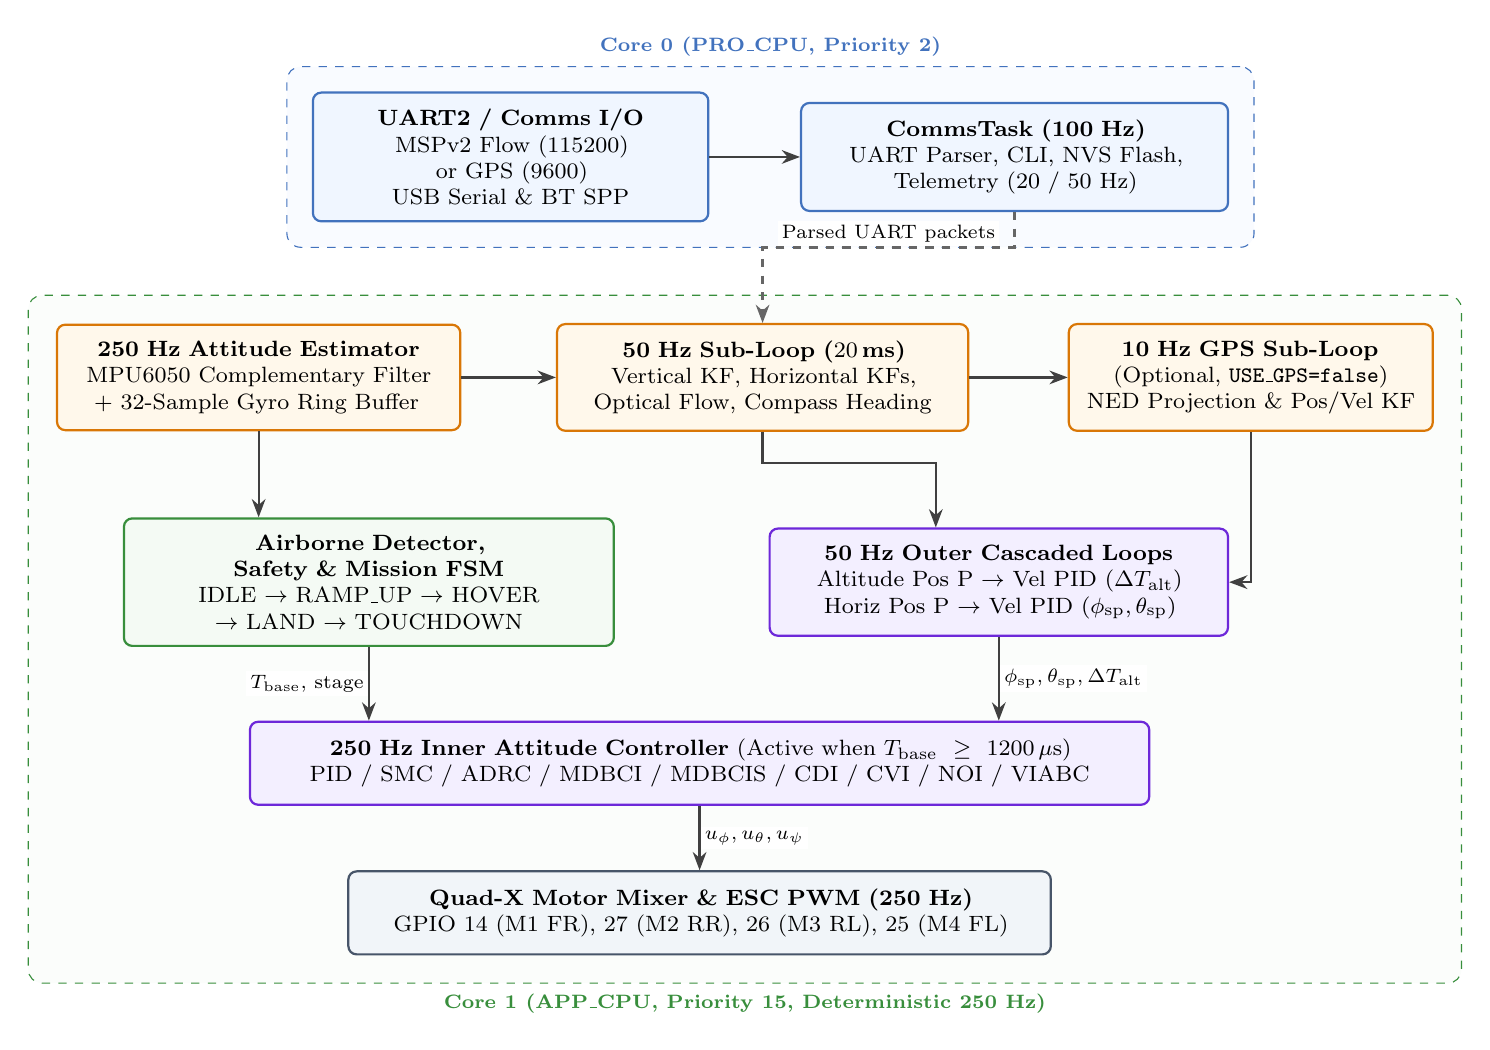
\begin{tikzpicture}[
  box/.style={
    rectangle, rounded corners=3pt, thick, align=center,
    font=\footnotesize, inner sep=6pt, minimum height=30pt
  }
]
  % Core 0 Row (y = 7.4)
  \node[box, draw=core0bd, fill=core0bg, text width=4.6cm] (uart) at (0, 7.4)
    {\textbf{UART2 / Comms I/O}\\MSPv2 Flow (115200) or GPS (9600)\\USB Serial \& BT SPP};
  \node[box, draw=core0bd, fill=core0bg, text width=5.0cm] (comms) at (6.4, 7.4)
    {\textbf{CommsTask (100~Hz)}\\UART Parser, CLI, NVS Flash,\\Telemetry (20 / 50~Hz)};

  % Core 1 Row 1: Estimators (y = 4.6)
  \node[box, draw=estbd, fill=estbg, text width=4.7cm] (att) at (-3.2, 4.6)
    {\textbf{250~Hz Attitude Estimator}\\MPU6050 Complementary Filter\\+ 32-Sample Gyro Ring Buffer};
  \node[box, draw=estbd, fill=estbg, text width=4.8cm] (sub50) at (3.2, 4.6)
    {\textbf{50~Hz Sub-Loop ($20\,\text{ms}$)}\\Vertical KF, Horizontal KFs,\\Optical Flow, Compass Heading};
  \node[box, draw=estbd, fill=estbg, text width=4.2cm] (sub10) at (9.4, 4.6)
    {\textbf{10~Hz GPS Sub-Loop}\\(Optional, \texttt{USE\_GPS=false})\\NED Projection \& Pos/Vel KF};

  % Core 1 Row 2: FSM & Outer Loops (y = 2.0)
  \node[box, draw=core1bd, fill=core1bg, text width=5.8cm] (fsm) at (-1.8, 2.0)
    {\textbf{Airborne Detector, Safety \& Mission FSM}\\IDLE $\rightarrow$ RAMP\_UP $\rightarrow$ HOVER $\rightarrow$ LAND $\rightarrow$ TOUCHDOWN};
  \node[box, draw=ctrlbd, fill=ctrlbg, text width=5.4cm] (outer) at (6.2, 2.0)
    {\textbf{50~Hz Outer Cascaded Loops}\\Altitude Pos P $\rightarrow$ Vel PID ($\Delta T_{\text{alt}}$)\\Horiz Pos P $\rightarrow$ Vel PID ($\phi_{\text{sp}}, \theta_{\text{sp}}$)};

  % Core 1 Row 3: Inner Controller (y = -0.3)
  \node[box, draw=ctrlbd, fill=ctrlbg, text width=11.0cm] (inner) at (2.4, -0.3)
    {\textbf{250~Hz Inner Attitude Controller} (Active when $T_{\text{base}} \ge 1200\,\mu\text{s}$)\\PID / SMC / ADRC / MDBCI / MDBCIS / CDI / CVI / NOI / VIABC};

  % Core 1 Row 4: Motor Mixer (y = -2.2)
  \node[box, draw=hwbd, fill=hwbg, text width=8.5cm] (mixer) at (2.4, -2.2)
    {\textbf{Quad-X Motor Mixer \& ESC PWM (250~Hz)}\\GPIO 14 (M1 FR), 27 (M2 RR), 26 (M3 RL), 25 (M4 FL)};

  % Arrows
  \draw[arrow] (uart) -- (comms);
  \draw[darrow] (comms.south) -- ++(0,-0.45) -| node[lbl, pos=0.25, above] {Parsed UART packets} (sub50.north);

  \draw[arrow] (att) -- (sub50);
  \draw[arrow] (sub50) -- (sub10);

  \draw[arrow] (att.south) -- (att.south |- fsm.north);
  \draw[arrow] (sub50.south) -- ++(0,-0.4) -| ([xshift=-0.8cm]outer.north);
  \draw[arrow] (sub10.south) |- (outer.east);

  \draw[arrow] (fsm.south) -- node[lbl, left] {$T_{\text{base}}$, stage} (fsm.south |- inner.north);
  \draw[arrow] (outer.south) -- node[lbl, right] {$\phi_{\text{sp}}, \theta_{\text{sp}}, \Delta T_{\text{alt}}$} (outer.south |- inner.north);
  \draw[arrow] (inner) -- node[lbl, right] {$u_\phi, u_\theta, u_\psi$} (mixer);

  % Background frames
  \begin{scope}[on background layer]
    \node[draw=core0bd, dashed, rounded corners=5pt, fill=core0bg!40, inner sep=9pt,
          fit=(uart)(comms),
          label={[font=\scriptsize\bfseries, color=core0bd]above:Core 0 (PRO\_CPU, Priority 2)}] {};
    \node[draw=core1bd, dashed, rounded corners=5pt, fill=core1bg!35, inner sep=10pt,
          fit=(att)(sub50)(sub10)(fsm)(outer)(inner)(mixer),
          label={[font=\scriptsize\bfseries, color=core1bd]below:Core 1 (APP\_CPU, Priority 15, Deterministic 250~Hz)}] {};
  \end{scope}
\end{tikzpicture}%
}
\caption{Dual-core FreeRTOS scheduling and multi-rate execution flow across Core~0 and Core~1.}
\label{fig:dual_core}
\end{figure}

% =============================================================================
\section{Hardware Sensors and Coordinate Conventions}
% =============================================================================

\subsection{Sensor Suite and Interfaces}
All sensors sit behind abstract C++ interfaces defined in \texttt{Sensors.h}: \texttt{IMUInterface}, \texttt{RangefinderInterface}, \texttt{BarometerInterface}, \texttt{CompassInterface}, \texttt{OpticalFlowInterface}, and \texttt{GPSInterface}. Table~\ref{tab:sensors} summarizes the hardware drivers and buses.

\begin{table}[htbp]
\centering
\small
\begin{tabularx}{\textwidth}{@{}ll>{\raggedright\arraybackslash}p{4.0cm}X@{}}
\toprule
\textbf{Subsystem} & \textbf{Hardware / Driver} & \textbf{Bus / Rate} & \textbf{Role in Firmware} \\
\midrule
IMU & MPU6050 (\texttt{0x68}) & I2C 400~kHz, 250~Hz read & 3-axis accel ($\pm 8g$), gyro ($\pm 500^\circ/\text{s}$), 44~Hz DLPF \\
Optical Flow \& ToF & Mateksys 3901-L0X & UART2 (RX~16, TX~17), 115200~baud & MSPv2 \texttt{0x1F02} flow, \texttt{0x1F01} VL53 ToF LiDAR ($0.03\text{--}2.00\,\text{m}$) \\
Compass & GY-87 (QMC5883P / HMC5883L) & I2C bypass, 50~Hz read & Tilt-compensated True North yaw reference \\
GPS (Legacy) & NEO-M8N (NMEA) & UART2 shared, 9600~baud, 10~Hz & Disabled by default (\texttt{USE\_GPS = false}) \\
Baro / Sharp IR & BMP180 / GP2Y0A & Dewired / Inactive & Bypassed when ToF LiDAR mode is enabled (\texttt{USE\_LIDAR\_ONLY\_ALTITUDE}) \\
\bottomrule
\end{tabularx}
\caption{Active sensor hardware and bus configuration defined in \texttt{Config.h} and \texttt{Sensors.cpp}.}
\label{tab:sensors}
\end{table}

\subsection{Body Frame Sign Conventions and Lever Arms}
The firmware uses a body-fixed frame where $+X$ points \textbf{Forward}, $+Y$ points \textbf{Right}, and $+Z$ points \textbf{Down} for physical lever-arm offsets relative to the center of mass (CM):
\begin{equation}
  \mathbf{r}_{\text{flow}} = \begin{bmatrix} -0.04 \\ +0.01 \\ +0.03 \end{bmatrix}\text{m}, \qquad
  \mathbf{r}_{\text{imu}}  = \begin{bmatrix} -0.02 \\ +0.02 \\ 0.00 \end{bmatrix}\text{m}.
\end{equation}
From \texttt{StateEstimator.cpp}, gyroscope rates after calibration bias subtraction and axis sign mapping satisfy:
\begin{align}
  g_x &= -(g_{x,\text{raw}} - b_{gx})\frac{180}{\pi} \quad(\text{right wing down} > 0), \\
  g_y &=  (g_{y,\text{raw}} - b_{gy})\frac{180}{\pi} \quad(\text{nose down} > 0), \\
  g_z &=  (g_{z,\text{raw}} - b_{gz})\frac{180}{\pi} \quad(\text{clockwise yaw} > 0).
\end{align}
Correspondingly, positive roll $\phi > 0$ tilts the right wing down, positive pitch $\theta > 0$ pitches the nose down (accelerating forward), and positive yaw $\psi > 0$ rotates clockwise when viewed from above.

% =============================================================================
\section{State Estimation Architecture}
% =============================================================================

State estimation is partitioned into three estimators: a 250~Hz attitude complementary filter, a 50~Hz 3-state vertical Kalman filter, and two decoupled 50~Hz 3-state horizontal Kalman filters fused with latency-compensated optical flow (and optional 10~Hz GPS). Figure~\ref{fig:state_est} summarizes the full estimation pipeline.

\begin{figure}[htbp]
\centering
\resizebox{\textwidth}{!}{%
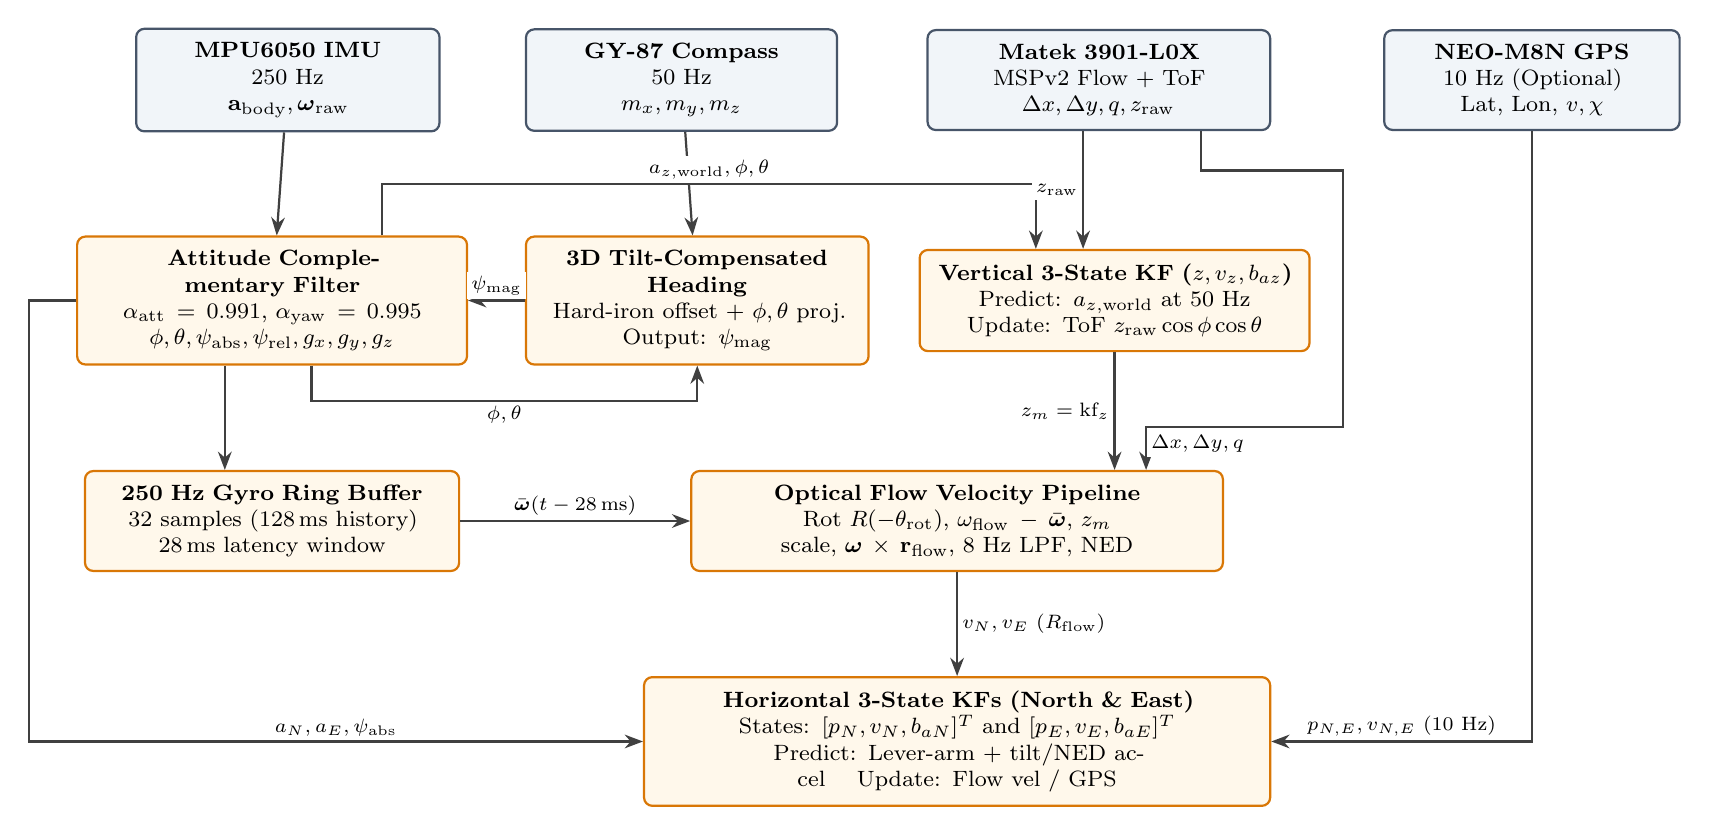
\begin{tikzpicture}[
  box/.style={
    rectangle, rounded corners=3pt, thick, align=center,
    font=\footnotesize, inner sep=5pt, minimum height=28pt
  }
]
  % Row 1 (y = 8.4): Raw Sensors
  \node[box, draw=hwbd, fill=hwbg, text width=3.5cm] (imu) at (0, 8.4)
    {\textbf{MPU6050 IMU}\\250~Hz\\$\mathbf{a}_{\text{body}}, \boldsymbol{\omega}_{\text{raw}}$};
  \node[box, draw=hwbd, fill=hwbg, text width=3.6cm] (mag) at (5.0, 8.4)
    {\textbf{GY-87 Compass}\\50~Hz\\$m_x, m_y, m_z$};
  \node[box, draw=hwbd, fill=hwbg, text width=4.0cm] (flow) at (10.3, 8.4)
    {\textbf{Matek 3901-L0X}\\MSPv2 Flow + ToF\\$\Delta x, \Delta y, q, z_{\text{raw}}$};
  \node[box, draw=hwbd, fill=hwbg, text width=3.4cm] (gps) at (15.8, 8.4)
    {\textbf{NEO-M8N GPS}\\10~Hz (Optional)\\Lat, Lon, $v, \chi$};

  % Row 2 (y = 5.6): Attitude, Compass, Vertical KF
  \node[box, draw=estbd, fill=estbg, text width=4.6cm] (attfilt) at (-0.2, 5.6)
    {\textbf{Attitude Complementary Filter}\\$\alpha_{\text{att}} = 0.991$, $\alpha_{\text{yaw}} = 0.995$\\$\phi, \theta, \psi_{\text{abs}}, \psi_{\text{rel}}, g_x, g_y, g_z$};
  \node[box, draw=estbd, fill=estbg, text width=4.0cm] (compass) at (5.2, 5.6)
    {\textbf{3D Tilt-Compensated Heading}\\Hard-iron offset + $\phi, \theta$ proj.\\Output: $\psi_{\text{mag}}$};
  \node[box, draw=estbd, fill=estbg, text width=4.6cm] (vkf) at (10.5, 5.6)
    {\textbf{Vertical 3-State KF ($z, v_z, b_{az}$)}\\Predict: $a_{z,\text{world}}$ at 50~Hz\\Update: ToF $z_{\text{raw}}\cos\phi\cos\theta$};

  % Row 3 (y = 2.8): Ring Buffer & Optical Flow Pipeline
  \node[box, draw=estbd, fill=estbg, text width=4.4cm] (ring) at (-0.2, 2.8)
    {\textbf{250~Hz Gyro Ring Buffer}\\32 samples ($128\,\text{ms}$ history)\\$28\,\text{ms}$ latency window};
  \node[box, draw=estbd, fill=estbg, text width=6.4cm] (ofpipe) at (8.5, 2.8)
    {\textbf{Optical Flow Velocity Pipeline}\\Rot $R(-\theta_{\text{rot}})$, $\omega_{\text{flow}} - \bar{\boldsymbol{\omega}}$, $z_m$ scale, $\boldsymbol{\omega}\times\mathbf{r}_{\text{flow}}$, 8~Hz LPF, NED};

  % Row 4 (y = 0.0): Horizontal KFs
  \node[box, draw=estbd, fill=estbg, text width=7.6cm] (hkf) at (8.5, 0.0)
    {\textbf{Horizontal 3-State KFs (North \& East)}\\States: $[p_N, v_N, b_{aN}]^T$ and $[p_E, v_E, b_{aE}]^T$\\Predict: Lever-arm + tilt/NED accel \quad Update: Flow vel / GPS};

  % Orthogonal Connections
  \draw[arrow] (imu) -- (attfilt);
  \draw[arrow] (mag) -- (compass);
  \draw[arrow] (compass.west) -- node[lbl, above] {$\psi_{\text{mag}}$} (attfilt.east);
  \draw[arrow] ([xshift=0.5cm]attfilt.south) -- ++(0,-0.45) -| node[lbl, pos=0.25, below] {$\phi, \theta$} (compass.south);
  \draw[arrow] ([xshift=-0.6cm]attfilt.south) -- ([xshift=-0.6cm]ring.north);

  % Attitude -> Vertical KF (routed cleanly above Row 2/3 gap)
  \draw[arrow] ([xshift=1.4cm]attfilt.north) -- ++(0, 0.65) -| node[lbl, pos=0.25, above] {$a_{z,\text{world}}, \phi, \theta$} ([xshift=-1.0cm]vkf.north);
  \draw[arrow] ([xshift=-0.2cm]flow.south) -- node[lbl, left] {$z_{\text{raw}}$} ([xshift=-0.4cm]vkf.north);

  % Flow + Ring + VKF -> Optical Flow Pipeline
  \draw[arrow] (ring.east) -- node[lbl, above] {$\bar{\boldsymbol{\omega}}(t - 28\,\text{ms})$} (ofpipe.west);
  \draw[arrow] ([xshift=1.3cm]flow.south) -- ++(0, -0.5) -| (13.4, 4.1) |- ([yshift=0.55cm, xshift=2.4cm]ofpipe.north) -- node[lbl, right, pos=0.4] {$\Delta x, \Delta y, q$} ([xshift=2.4cm]ofpipe.north);
  \draw[arrow] (vkf.south) -- node[lbl, left] {$z_m = \text{kf}_z$} (vkf.south |- ofpipe.north);

  % Optical Flow + Attitude + GPS -> Horizontal KFs
  \draw[arrow] (ofpipe.south) -- node[lbl, right] {$v_N, v_E$ ($R_{\text{flow}}$)} (hkf.north);
  \draw[arrow] (attfilt.west) -- ++(-0.6, 0) |- node[lbl, pos=0.75, above] {$a_N, a_E, \psi_{\text{abs}}$} (hkf.west);
  \draw[arrow] (gps.south) |- node[lbl, pos=0.75, above] {$p_{N,E}, v_{N,E}$ (10~Hz)} (hkf.east);
\end{tikzpicture}%
}
\caption{Multi-rate sensor fusion and state estimation dataflow across attitude, vertical, and horizontal estimators.}
\label{fig:state_est}
\end{figure}

\subsection{Attitude Complementary Filter (250~Hz)}
At each $4\,\text{ms}$ step, calibrated accelerometer angles are computed as:
\begin{equation}
  \phi_{\text{acc}} = \operatorname{atan2}\!\left(a_y, \sqrt{a_x^2 + a_z^2}\right)\frac{180}{\pi}, \qquad
  \theta_{\text{acc}} = \operatorname{atan2}\!\left(a_x, \sqrt{a_y^2 + a_z^2}\right)\frac{180}{\pi}.
\end{equation}
Roll and pitch fuse gyro integration with accelerometer tilt ($\alpha_{\text{att}} = 0.991$):
\begin{align}
  \phi_k   &= \alpha_{\text{att}}\left(\phi_{k-1} + g_x \Delta t\right) + (1 - \alpha_{\text{att}})\left(\phi_{\text{acc}} - \phi_{\text{cal}}\right), \\
  \theta_k &= \alpha_{\text{att}}\left(\theta_{k-1} + g_y \Delta t\right) + (1 - \alpha_{\text{att}})\left(\theta_{\text{acc}} - \theta_{\text{cal}}\right).
\end{align}
Compass readings (updated at 50~Hz) subtract hard-iron biases $(m_{x0}, m_{y0}, m_{z0})$ and project onto the horizontal plane using $(\phi + \phi_{\text{cal}}, \theta + \theta_{\text{cal}})$:
\begin{align}
  X_h &= m_x \cos\theta + m_y \sin\phi\sin\theta + m_z \cos\phi\sin\theta, \qquad
  Y_h = m_y \cos\phi - m_z \sin\phi, \\
  \psi_{\text{mag}} &= \operatorname{atan2}(Y_h, X_h)\frac{180}{\pi} + \delta_{\text{mag}}.
\end{align}
Absolute heading fuses gyro $g_z$ with $\psi_{\text{mag}}$ ($\alpha_{\text{yaw}} = 0.995$), wrapped to $[-180^\circ, 180^\circ]$:
\begin{equation}
  \psi_{\text{abs},k} = \psi_{\text{abs},k-1} + g_z \Delta t + (1 - \alpha_{\text{yaw}})\,\operatorname{wrap}_{180}(\psi_{\text{mag}} - \psi_{\text{abs},k-1}), \qquad
  \psi_{\text{rel}} = \operatorname{wrap}_{180}(\psi_{\text{abs}} - \psi_{\text{offset}}).
\end{equation}
Crucially, NED world-frame projections for horizontal estimation and position control use $\psi_{\text{abs}}$, whereas yaw damping uses body rate $g_z$.

\subsection{3-State Vertical Kalman Filter (50~Hz)}
The vertical estimator tracks $\mathbf{x}_z = [z,\ v_z,\ b_{az}]^T$ (altitude in $\text{m}$, climb rate in $\text{m/s}$, and vertical accelerometer bias in $\text{m/s}^2$). World vertical acceleration removes gravity along the tilted body axes:
\begin{equation}
  a_{z,\text{world}} = a_x \sin\theta - a_y \sin\phi\cos\theta + a_z \cos\phi\cos\theta - 9.80665.
\end{equation}
When airborne (or in simulation mode), the prediction step propagates with $a_{\text{corr}} = a_{z,\text{world}} - b_{az}$ and state transition matrix $\mathbf{F}_z$:
\begin{equation}
  \mathbf{x}_{z,k|k-1} = \begin{bmatrix} 1 & \Delta t & -\frac{1}{2}\Delta t^2 \\ 0 & 1 & -\Delta t \\ 0 & 0 & 1 \end{bmatrix} \mathbf{x}_{z,k-1} + \begin{bmatrix} \frac{1}{2}\Delta t^2 \\ \Delta t \\ 0 \end{bmatrix} a_{z,\text{world}}, \qquad
  \mathbf{Q}_z = \operatorname{diag}(0.0002,\; 0.0035,\; 0.00003).
\end{equation}
Prior to airborne liftoff confirmation, $z$ tracks the ground baseline or valid ToF reading directly with $v_z = b_{az} = 0$ and primed covariance $\mathbf{P}_z = \operatorname{diag}(0.01, 0.05, 0.01)$. The Mateksys VL53 ToF LiDAR measurement is tilt-compensated:
\begin{equation}
  z_{\text{rf}} = z_{\text{raw}} \cos\phi \cos\theta,
\end{equation}
and accepted when LiDAR quality $> 30$, $|\phi|,|\theta| \le 35^\circ$, and $0.03 \le z_{\text{rf}} \le 2.00\,\text{m}$. Scalar Kalman updates use measurement matrix $\mathbf{H} = [1\ 0\ 0]$ and variance $R_{\text{lidar}} = 0.0025\,\text{m}^2$, clamping $|b_{az}| \le 2.0\,\text{m/s}^2$.

\subsection{Horizontal 3-State Kalman Filters and Optical Flow Pipeline (50~Hz)}
Two identical 1D 3-state Kalman filters (\texttt{kfNorth}, \texttt{kfEast}) estimate $\mathbf{x}_h = [p,\ v,\ b_a]^T$ along Earth North and East using $\mathbf{Q}_h = \operatorname{diag}(0.005, 0.035, 0.0005)$.

\subsubsection*{Inertial Prediction Step}
First, IMU centrifugal acceleration from yaw rate $g_z$ (in $\text{rad/s}$) due to CM offset $(r_{\text{imu},x}, r_{\text{imu},y})$ is compensated, gravity projections are canceled, and calibrated static offsets are subtracted:
\begin{align}
  a_{x,\text{cm}} &= a_x + g_z^2 r_{\text{imu},x}, & a_{y,\text{cm}} &= a_y + g_z^2 r_{\text{imu},y}, \\
  a_{\text{fwd}}   &= a_{x,\text{cm}}\cos\theta - a_z\sin\theta - a_{\text{fwd},0}, &
  a_{\text{right}} &= a_{y,\text{cm}}\cos\phi   - a_z\sin\phi   - a_{\text{right},0}.
\end{align}
Rotating into Earth NED via $\psi_{\text{abs}}$ gives $a_N = a_{\text{fwd}}\cos\psi_{\text{abs}} - a_{\text{right}}\sin\psi_{\text{abs}}$ and $a_E = a_{\text{fwd}}\sin\psi_{\text{abs}} + a_{\text{right}}\cos\psi_{\text{abs}}$. Inside \texttt{predict()}, bias-corrected acceleration $a_{\text{corr}} = a_{\text{meas}} - b_a$ applies a noise-floor deadband ($|a_{\text{corr}}| < 0.015\,\text{m/s}^2 \Rightarrow 0$) and velocity clamp $|v| \le 6.0\,\text{m/s}$. While resting on the ground, states are held at zero to prevent stationary drift.

\subsubsection*{Optical Flow Velocity Measurement Update}
When a new MSPv2 \texttt{0x1F02} packet arrives with surface tracking quality $q \ge 35$, the optical flow estimator (\texttt{updateOpticalFlowEstimator()}) executes six stages:
\begin{enumerate}
  \item \textbf{Latency-Matched Gyro Window:} Extracts delayed gyro averages $(\bar{g}_x, \bar{g}_y, \bar{g}_z)$ from the 250~Hz 32-sample ring buffer shifted back by $\text{round}(\text{FLOW\_DELAY\_MS}/4\,\text{ms}) = 7$ samples ($28\,\text{ms}$) across the flow integration window ($\approx 5$ samples for $20\,\text{ms}$).
  \item \textbf{Mounting Rotation \& Scaling:} Rotates raw counts $(s_x, s_y)$ by $-\theta_{\text{rot}}$ (default $90^\circ$) into body Forward/Right counts and scales by $s_{\text{rad}} = 0.00380\,\text{rad/count}$:
  \begin{equation}
    \omega_{\text{flow},x} = \frac{s_x\cos\theta_{\text{rot}} - s_y\sin\theta_{\text{rot}}}{\Delta t}\,s_{\text{rad}}, \qquad
    \omega_{\text{flow},y} = \frac{s_x\sin\theta_{\text{rot}} + s_y\cos\theta_{\text{rot}}}{\Delta t}\,s_{\text{rad}}.
  \end{equation}
  \item \textbf{Gyro Derotation \& Height Scaling:} Subtracts body angular rates (matching sign conventions: nose-down $\bar{g}_y$ and forward translation sweep ground features identically) and scales by clamped vertical KF height $z_m \in [0.05, 3.00]\,\text{m}$:
  \begin{equation}
    v_{\text{sens,fwd}} = (\omega_{\text{flow},x} - \bar{g}_y)z_m, \qquad
    v_{\text{sens,right}} = (\omega_{\text{flow},y} - \bar{g}_x)z_m.
  \end{equation}
  \item \textbf{Rigid-Body Lever-Arm Compensation:} Removes tangential velocity $\boldsymbol{\omega} \times \mathbf{r}_{\text{flow}}$ caused by rotation about the CM (with nose-up rate $q_{\text{up}} = -\bar{g}_y$):
  \begin{equation}
    v_{\text{raw,fwd}}   = v_{\text{sens,fwd}}   - (q_{\text{up}} r_{z} - \bar{g}_z r_{y}), \qquad
    v_{\text{raw,right}} = v_{\text{sens,right}} - (\bar{g}_z r_{x} - \bar{g}_x r_{z}),
  \end{equation}
  clamped to $\pm 3.5\,\text{m/s}$.
  \item \textbf{Low-Pass Filter \& NED Rotation:} Filters body velocities with a 1st-order exponential LPF ($\alpha = 1 - e^{-2\pi f_c \Delta t}$, $f_c = 8.0\,\text{Hz}$) and rotates by $\psi_{\text{abs}}$ to $(v_N, v_E)$.
  \item \textbf{Quality-Adaptive Kalman Update:} Updates \texttt{kfNorth.updateVel} and \texttt{kfEast.updateVel} when airborne or in sim mode using quality-scaled variance:
  \begin{equation}
    R_{\text{flow}} = \operatorname{clamp}\!\left(\frac{2 R_{\text{flow},0}}{q / 255},\; 0.015,\; 0.40\right), \qquad R_{\text{flow},0} = 0.02\,\text{m}^2/\text{s}^2.
  \end{equation}
\end{enumerate}

When GPS is enabled (\texttt{updatePositionEstimator()} at 10~Hz with $\ge 5$ satellites and $\text{HDOP} \le 4.0$), flat-Earth lat/lon offsets update position with $R_{\text{pos}} = \operatorname{clamp}(0.4\,\text{HDOP}^2, 0.4, 15.0)$ and Doppler velocity updates velocity with $R_{\text{vel}} = 0.08$.

% =============================================================================
\section{Autonomous Flight Mission State Machine and Safety Guards}
% =============================================================================

Before the inner attitude loop computes motor commands, Core~1 evaluates airborne detection, safety overrides, and the 5-stage autonomous mission state machine (\texttt{balance\_controller.ino}).

\begin{figure}[htbp]
\centering
\resizebox{\textwidth}{!}{%
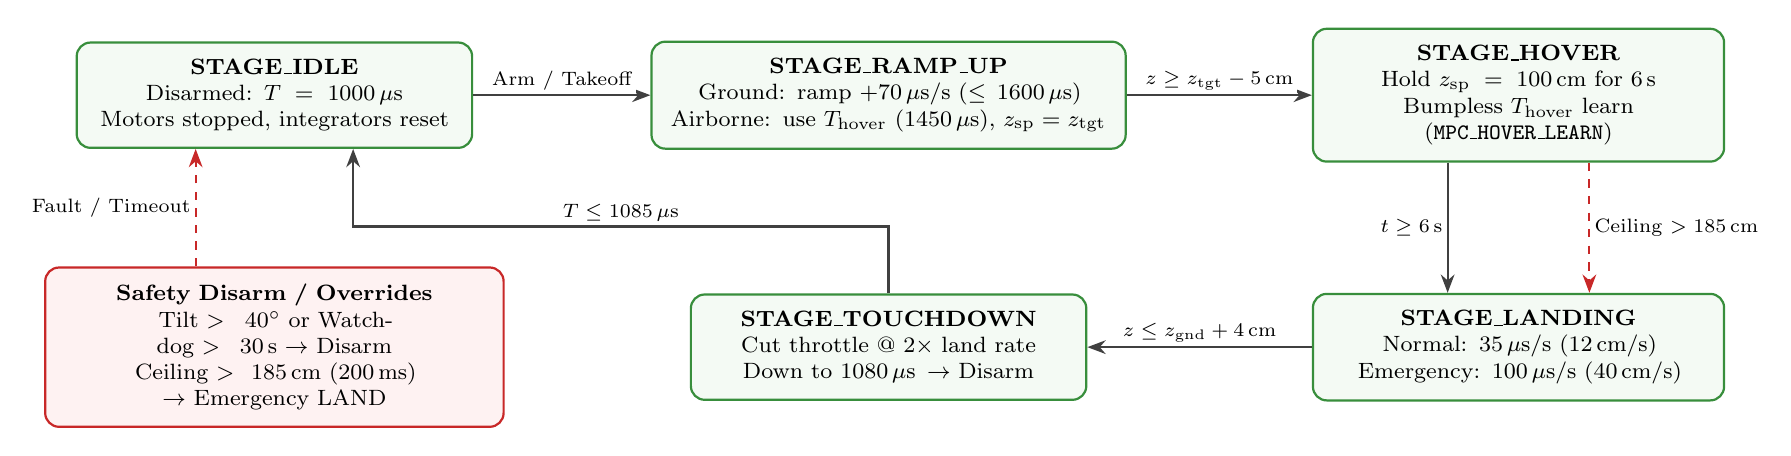
\begin{tikzpicture}[
  box/.style={
    rectangle, rounded corners=5pt, thick, align=center,
    font=\footnotesize, inner sep=6pt, minimum height=34pt
  }
]
  % Row 1 (y = 3.2)
  \node[box, draw=core1bd, fill=core1bg, text width=4.6cm] (idle) at (0, 3.2)
    {\textbf{STAGE\_IDLE}\\Disarmed: $T = 1000\,\mu\text{s}$\\Motors stopped, integrators reset};
  \node[box, draw=core1bd, fill=core1bg, text width=5.6cm] (ramp) at (7.8, 3.2)
    {\textbf{STAGE\_RAMP\_UP}\\Ground: ramp $+70\,\mu\text{s/s}$ ($\le 1600\,\mu\text{s}$)\\Airborne: use $T_{\text{hover}}$ ($1450\,\mu\text{s}$), $z_{\text{sp}} = z_{\text{tgt}}$};
  \node[box, draw=core1bd, fill=core1bg, text width=4.8cm] (hover) at (15.8, 3.2)
    {\textbf{STAGE\_HOVER}\\Hold $z_{\text{sp}} = 100\,\text{cm}$ for $6\,\text{s}$\\Bumpless $T_{\text{hover}}$ learn (\texttt{MPC\_HOVER\_LEARN})};

  % Row 2 (y = 0.0)
  \node[box, draw=safebd, fill=safebg, text width=5.4cm] (safe) at (0, 0.0)
    {\textbf{Safety Disarm / Overrides}\\Tilt $> 40^\circ$ or Watchdog $> 30\,\text{s}$ $\rightarrow$ Disarm\\Ceiling $> 185\,\text{cm}$ ($200\,\text{ms}$) $\rightarrow$ Emergency LAND};
  \node[box, draw=core1bd, fill=core1bg, text width=4.6cm] (touch) at (7.8, 0.0)
    {\textbf{STAGE\_TOUCHDOWN}\\Cut throttle @ $2\times$ land rate\\Down to $1080\,\mu\text{s} \rightarrow$ Disarm};
  \node[box, draw=core1bd, fill=core1bg, text width=4.8cm] (land) at (15.8, 0.0)
    {\textbf{STAGE\_LANDING}\\Normal: $35\,\mu\text{s/s}$ ($12\,\text{cm/s}$)\\Emergency: $100\,\mu\text{s/s}$ ($40\,\text{cm/s}$)};

  % Orthogonal State Transitions
  \draw[arrow] (idle) -- node[lbl, above] {Arm / Takeoff} (ramp);
  \draw[arrow] (ramp) -- node[lbl, above] {$z \ge z_{\text{tgt}} - 5\,\text{cm}$} (hover);
  \draw[arrow] ([xshift=-0.9cm]hover.south) -- node[lbl, left] {$t \ge 6\,\text{s}$} ([xshift=-0.9cm]land.north);
  \draw[arrow] (land) -- node[lbl, above] {$z \le z_{\text{gnd}} + 4\,\text{cm}$} (touch);
  \draw[arrow] (touch.north) -- ++(0, 0.85) -| node[lbl, pos=0.25, above] {$T \le 1085\,\mu\text{s}$} ([xshift=1.0cm]idle.south);

  % Safety Overrides
  \draw[darrow, draw=safebd] ([xshift=0.9cm]hover.south) -- node[lbl, right] {Ceiling $> 185\,\text{cm}$} ([xshift=0.9cm]land.north);
  \draw[darrow, draw=safebd] ([xshift=-1.0cm]safe.north) -- node[lbl, left] {Fault / Timeout} ([xshift=-1.0cm]idle.south);
\end{tikzpicture}%
}
\caption{Autonomous flight mission state machine, airborne liftoff handoff, and safety overrides.}
\label{fig:mission_fsm}
\end{figure}

\noindent Key operational rules in the mission manager:
\begin{itemize}
  \item \textbf{Debounced Airborne Confirmation:} While armed with $T_{\text{base}} \ge 1260\,\mu\text{s}$, liftoff is declared if fused height exceeds $z_{\text{gnd}} + 5\,\text{cm}$ or valid LiDAR exceeds $z_{\text{gnd}} + 4\,\text{cm}$ continuously for $150\,\text{ms}$ (fallback: $T_{\text{base}} \ge 1480\,\mu\text{s}$ sustained for $600\,\text{ms}$). Upon confirmation, open-loop ramping stops, $T_{\text{hover}}$ keeps the configured \texttt{MPC\_THR\_HOVER} ($1450\,\mu\text{s}$), and \texttt{alt\_throttle\_adj} is seeded with $T_{\text{curr}} - T_{\text{hover}}$ for a bumpless handoff.
  \item \textbf{In-Flight Hover Thrust Learning (\texttt{MPC\_HOVER\_LEARN}):} When enabled during \texttt{STAGE\_HOVER} and steady ($|z - z_{\text{tgt}}| < 5\,\text{cm}$, $|v_z| < 0.12\,\text{m/s}$), $5\%$ per second of \texttt{alt\_throttle\_adj} is accumulated in a float and transferred bumplessly from $I_{vz}$ into $T_{\text{hover}} \in [1150, 1700]\,\mu\text{s}$, saving to NVS \texttt{MPC\_THR\_HOVER} after $2.0\,\text{s}$.
  \item \textbf{Separate Normal \& Emergency Descent:} Normal landings (\texttt{land} or hover completion) descend at \texttt{MPC\_RAMP\_DN} ($35\,\mu\text{s/s}$, $12\,\text{cm/s}$). Toggling \texttt{start} in flight, \texttt{stop}, or ceiling intervention triggers an emergency descent at \texttt{MPC\_RAMP\_EMG} ($100\,\mu\text{s/s}$, $40\,\text{cm/s}$).
  \item \textbf{Closed-Loop Activation \& Anti-Windup:} Attitude controllers stay reset while $T_{\text{base}} < 1200\,\mu\text{s}$ (\texttt{PID\_ACTIVE\_THROTTLE}). Integral and ESO disturbance terms only accumulate when \texttt{run\_iterm = sim\_mode || is\_airborne}.
\end{itemize}

% =============================================================================
\section{Cascaded Control Architecture}
% =============================================================================

Figure~\ref{fig:cascade_overview} shows the full cascaded control hierarchy connecting the 50~Hz outer position and altitude loops to the 250~Hz inner attitude loop and Quad-X mixer.

\begin{figure}[htbp]
\centering
\resizebox{\textwidth}{!}{%
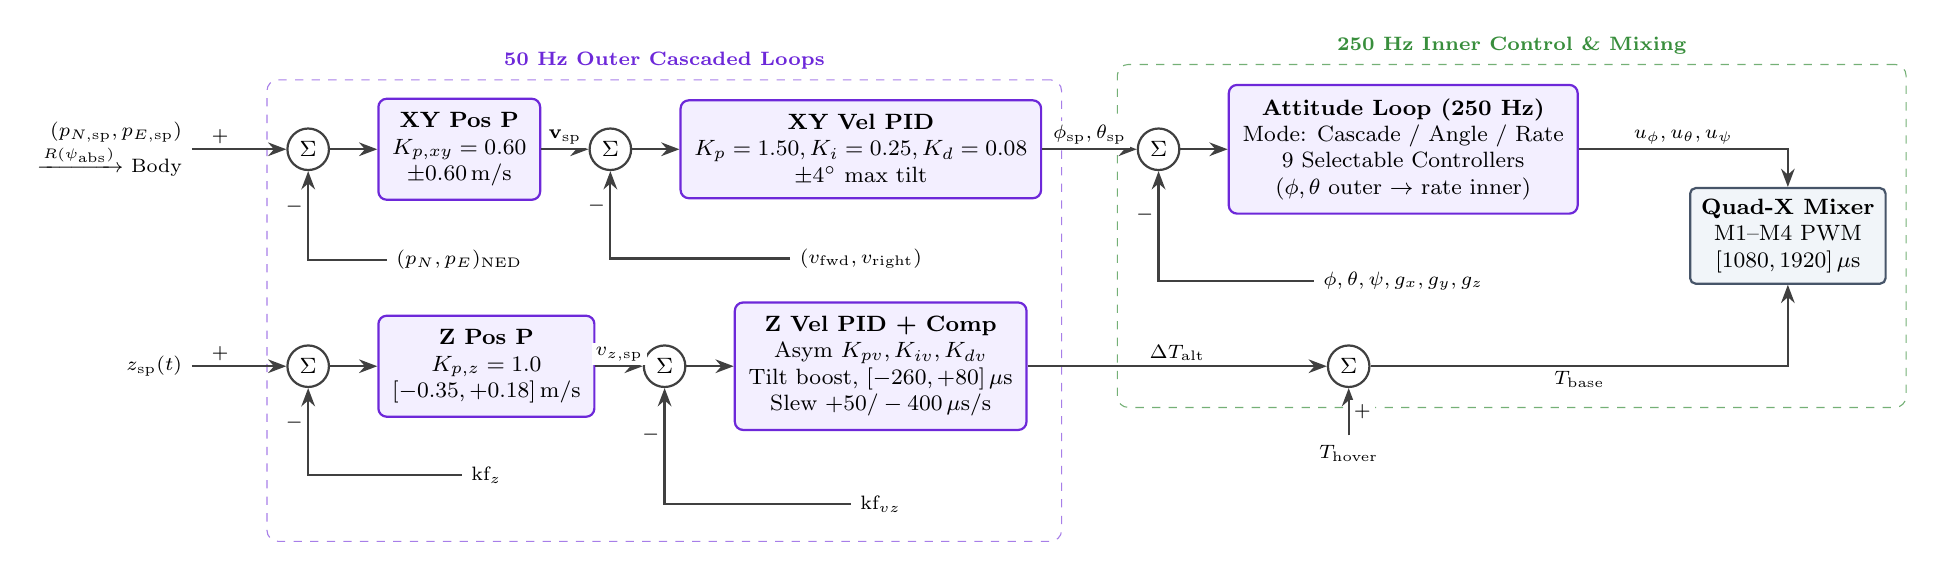
\begin{tikzpicture}[node distance=5mm and 6mm]
  % Horizontal Position Cascade (Top branch)
  \node[sum] (sum_pos) {$\Sigma$};
  \node[controller, right=of sum_pos] (pos_p) {\textbf{XY Pos P}\\$K_{p,xy}=0.60$\\$\pm 0.60\,\text{m/s}$};
  \node[sum, right=of pos_p] (sum_vel) {$\Sigma$};
  \node[controller, right=of sum_vel] (vel_pid) {\textbf{XY Vel PID}\\$K_p=1.50, K_i=0.25, K_d=0.08$\\$\pm 4^\circ$ max tilt};

  % Vertical Altitude Cascade (Bottom branch)
  \node[sum, below=22mm of sum_pos] (sum_z) {$\Sigma$};
  \node[controller, right=of sum_z] (z_p) {\textbf{Z Pos P}\\$K_{p,z}=1.0$\\$[-0.35, +0.18]\,\text{m/s}$};
  \node[sum, right=of z_p] (sum_vz) {$\Sigma$};
  \node[controller, right=of sum_vz] (vz_pid) {\textbf{Z Vel PID + Comp}\\Asym $K_{pv}, K_{iv}, K_{dv}$\\Tilt boost, $[-260,+80]\,\mu\text{s}$\\Slew $+50 / -400\,\mu\text{s/s}$};

  % Inner Attitude Cascade (Right side)
  \node[sum, right=12mm of vel_pid] (sum_ang) {$\Sigma$};
  \node[controller, right=of sum_ang] (ang_ctrl) {\textbf{Attitude Loop (250~Hz)}\\Mode: Cascade / Angle / Rate\\9 Selectable Controllers\\($\phi, \theta$ outer $\rightarrow$ rate inner)};
  \node[sum, right=10mm of vz_pid, xshift=28mm] (sum_thr) {$\Sigma$};
  \node[sensor, right=14mm of ang_ctrl, yshift=-11mm] (mix) {\textbf{Quad-X Mixer}\\M1--M4 PWM\\$[1080, 1920]\,\mu\text{s}$};

  % Labels for setpoints
  \node[left=12mm of sum_pos, font=\scriptsize, align=right] (sp_xy) {$(p_{N,\text{sp}}, p_{E,\text{sp}})$\\$\xrightarrow{R(\psi_{\text{abs}})}$ Body};
  \node[left=12mm of sum_z, font=\scriptsize, align=right] (sp_z) {$z_{\text{sp}}(t)$};

  % Connections XY
  \draw[arrow] (sp_xy) -- node[lbl, above, pos=0.3] {$+$} (sum_pos);
  \draw[arrow] (sum_pos) -- (pos_p);
  \draw[arrow] (pos_p) -- node[lbl, above] {$\mathbf{v}_{\text{sp}}$} (sum_vel);
  \draw[arrow] (sum_vel) -- (vel_pid);
  \draw[arrow] (vel_pid) -- node[lbl, above] {$\phi_{\text{sp}}, \theta_{\text{sp}}$} (sum_ang);

  % Connections Z
  \draw[arrow] (sp_z) -- node[lbl, above, pos=0.3] {$+$} (sum_z);
  \draw[arrow] (sum_z) -- (z_p);
  \draw[arrow] (z_p) -- node[lbl, above] {$v_{z,\text{sp}}$} (sum_vz);
  \draw[arrow] (sum_vz) -- (vz_pid);
  \draw[arrow] (vz_pid) -- node[lbl, above] {$\Delta T_{\text{alt}}$} (sum_thr);
  \node[below=6mm of sum_thr, font=\scriptsize] (t_base) {$T_{\text{hover}}$};
  \draw[arrow] (t_base) -- node[lbl, right] {$+$} (sum_thr);

  % Inner to Mixer
  \draw[arrow] (sum_ang) -- (ang_ctrl);
  \draw[arrow] (ang_ctrl.east) -| node[lbl, above, pos=0.25] {$u_\phi, u_\theta, u_\psi$} (mix.north);
  \draw[arrow] (sum_thr.east) -| node[lbl, below, pos=0.25] {$T_{\text{base}}$} (mix.south);

  % Feedback lines
  \node[below=5mm of pos_p, font=\scriptsize] (fb_xy) {$(p_N, p_E)_{\text{NED}}$};
  \draw[arrow] (fb_xy.west) -| node[lbl, left, pos=0.8] {$-$} (sum_pos.south);
  \node[below=5mm of vel_pid, font=\scriptsize] (fb_vxy) {$(v_{\text{fwd}}, v_{\text{right}})$};
  \draw[arrow] (fb_vxy.west) -| node[lbl, left, pos=0.8] {$-$} (sum_vel.south);

  \node[below=5mm of z_p, font=\scriptsize] (fb_z) {$\text{kf}_z$};
  \draw[arrow] (fb_z.west) -| node[lbl, left, pos=0.8] {$-$} (sum_z.south);
  \node[below=7mm of vz_pid, font=\scriptsize] (fb_vz) {$\text{kf}_{vz}$};
  \draw[arrow] (fb_vz.west) -| node[lbl, left, pos=0.8] {$-$} (sum_vz.south);

  \node[below=6mm of ang_ctrl, font=\scriptsize] (fb_att) {$\phi, \theta, \psi, g_x, g_y, g_z$};
  \draw[arrow] (fb_att.west) -| node[lbl, left, pos=0.8] {$-$} (sum_ang.south);

  % Loop rate frames
  \begin{scope}[on background layer]
    \node[draw=ctrlbd!60, dashed, rounded corners=4pt, inner sep=7pt,
          fit=(sum_pos)(vel_pid)(sum_z)(vz_pid)(fb_z)(fb_vz),
          label={[font=\scriptsize\bfseries, color=ctrlbd]above:50~Hz Outer Cascaded Loops}] {};
    \node[draw=core1bd!70, dashed, rounded corners=4pt, inner sep=7pt,
          fit=(sum_ang)(ang_ctrl)(sum_thr)(mix)(fb_att),
          label={[font=\scriptsize\bfseries, color=core1bd]above:250~Hz Inner Control \& Mixing}] {};
  \end{scope}
\end{tikzpicture}%
}
\caption{End-to-end cascaded flight control architecture from position/altitude outer loops to Quad-X motor mixing.}
\label{fig:cascade_overview}
\end{figure}

\subsection{Outer Horizontal Position Cascade (50~Hz)}
Implemented in \texttt{computePositionControl()} when position hold is active and either Optical Flow or a GPS home lock is available:
\begin{enumerate}
  \item \textbf{Setpoint Latch \& NED-to-Body Rotation:} Upon activation, the current NED position $(p_N, p_E)$ is latched as $(p_{N,\text{sp}}, p_{E,\text{sp}})$. Position errors and filtered NED velocities are rotated into body Forward/Right coordinates via $\psi_{\text{abs}}$:
  \begin{equation}
    \begin{bmatrix} e_{\text{fwd}} \\ e_{\text{right}} \end{bmatrix} =
    \begin{bmatrix} \cos\psi_{\text{abs}} & \sin\psi_{\text{abs}} \\ -\sin\psi_{\text{abs}} & \cos\psi_{\text{abs}} \end{bmatrix}
    \begin{bmatrix} p_{N,\text{sp}} - p_N \\ p_{E,\text{sp}} - p_E \end{bmatrix}.
  \end{equation}
  \item \textbf{Outer Position P Loop:} Desired body velocities are $v_{\text{sp}} = \operatorname{clamp}(K_{p,xy} e, -v_{\max}, v_{\max})$ with $K_{p,xy} = 0.60\,\text{s}^{-1}$ and $v_{\max} = 0.60\,\text{m/s}$ (active when airborne and $z \ge z_{\text{gnd}} + 9\,\text{cm}$).
  \item \textbf{Inner Velocity PID Loop:} Velocity errors $e_v = v_{\text{sp}} - v$ drive desired tilt angles directly in degrees (positive pitch nose-down accelerates forward; positive roll right-wing-down accelerates right):
  \begin{equation}
    \theta_{\text{sp}} = \operatorname{clamp}\!\left(K_{p,v} e_{v,\text{fwd}} + I_{\text{fwd}} - K_{d,v} \dot{v}_{\text{fwd}},\; -\theta_{\max},\; \theta_{\max}\right),
  \end{equation}
  with $K_{p,v} = 1.50^\circ/(\text{m/s})$, $K_{i,v} = 0.25^\circ/\text{m}$ (clamped at $\pm 1.5^\circ$), $K_{d,v} = 0.08$ (derivative clamped $\pm 2.0^\circ$), and $\theta_{\max} = 4.0^\circ$. An identical law computes $\phi_{\text{sp}}$ on the Right axis.
\end{enumerate}

\subsection{Outer Vertical Altitude Cascade (50~Hz)}
Implemented in \texttt{computeAltitudeControl()}:
\begin{enumerate}
  \item \textbf{Outer Z Position P Loop:} $v_{z,\text{sp}} = \operatorname{clamp}(K_{p,z}(z_{\text{sp}} - z), -v_{\text{desc},\max}, v_{\text{climb},\max})$ with $K_{p,z} = 1.0\,\text{s}^{-1}$, $v_{\text{climb},\max} = 0.18\,\text{m/s}$, and $v_{\text{desc},\max} = 0.35\,\text{m/s}$. The acceleration-to-PWM scale factor uses the nominal hover baseline $T_{\text{hover}} - 1000$ rather than $T_{\text{base}} - 1000$.
  \item \textbf{Inner Z Velocity PID with Asymmetric Gains:} Using $e_{vz} = v_{z,\text{sp}} - v_z$:
  \begin{align}
    a_{z,\text{sp}} &= K_{p,\text{eff}}\, e_{vz} + I_{vz} - K_{d,vz}\frac{v_{z,k} - v_{z,k-1}}{\Delta t}, \\
    K_{p,\text{eff}} &= \begin{cases} K_{p,vz} = 1.8 & e_{vz} \ge 0\text{ (climb)}, \\ 2 K_{p,vz} = 3.6 & e_{vz} < 0\text{ (brake/descend)}. \end{cases}
  \end{align}
  The integrator ($K_{i,vz} = 0.50$, clamped $[-2.5, 1.2]$) freezes positive accumulation and decays at $2.0/\text{s}$ whenever the drone is above target ($e_z < -0.04\,\text{m}$).
  \item \textbf{Throttle Mapping, Tilt Compensation, and Asymmetric Slew Limit:} Acceleration maps to PWM via $\Delta T_{\text{raw}} = a_{z,\text{sp}} \cdot \frac{T_{\text{base}} - 1000}{9.80665}$, plus tilt-thrust boost $\left(\frac{1}{\cos\phi\cos\theta}-1\right)(T_{\text{base}}-1000)$ (clamped $+60\,\mu\text{s}$ and attenuated above target). Authority is clamped asymmetrically to $[-260, +80]\,\mu\text{s}$ (with extra emergency cut above $z_{\text{tgt}}+25\,\text{cm}$ or $180\,\text{cm}$), then slew-limited to $+50\,\mu\text{s/s}$ upward and $-400\,\mu\text{s/s}$ downward ($-600\,\mu\text{s/s}$ in ceiling emergency).
\end{enumerate}

% =============================================================================
\section{Inner Attitude Controllers (250~Hz) and Flight Modes}
% =============================================================================

All nine attitude controllers inherit from \texttt{AttitudeController} and support three flight modes (\texttt{MODE\_CASCADE} default, \texttt{MODE\_ANGLE}, and \texttt{MODE\_RATE}), switchable via \texttt{ctrl <name>}. Figure~\ref{fig:att_controllers} shows the routing across flight modes and controller laws.

\begin{figure}[htbp]
\centering
\resizebox{\textwidth}{!}{%
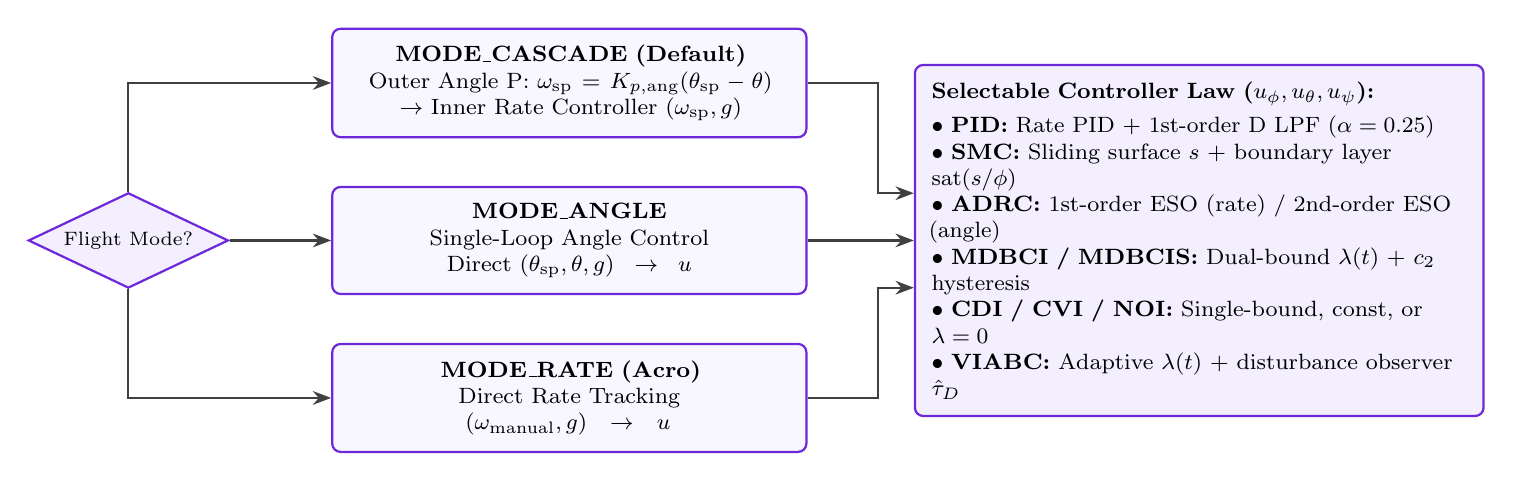
\begin{tikzpicture}[
  box/.style={
    rectangle, rounded corners=3pt, thick, align=center,
    font=\footnotesize, inner sep=6pt, minimum height=28pt
  }
]
  \node[decision] (mode) at (0, 0) {Flight Mode?};

  \node[box, draw=ctrlbd, fill=ctrlbg!55, text width=5.6cm] (casc) at (5.6, 2.0)
    {\textbf{MODE\_CASCADE (Default)}\\Outer Angle P: $\omega_{\text{sp}} = K_{p,\text{ang}}(\theta_{\text{sp}} - \theta)$\\$\rightarrow$ Inner Rate Controller $(\omega_{\text{sp}}, g)$};
  \node[box, draw=ctrlbd, fill=ctrlbg!55, text width=5.6cm] (ang) at (5.6, 0.0)
    {\textbf{MODE\_ANGLE}\\Single-Loop Angle Control\\Direct $(\theta_{\text{sp}}, \theta, g) \rightarrow u$};
  \node[box, draw=ctrlbd, fill=ctrlbg!55, text width=5.6cm] (rate) at (5.6, -2.0)
    {\textbf{MODE\_RATE (Acro)}\\Direct Rate Tracking\\$(\omega_{\text{manual}}, g) \rightarrow u$};

  \node[box, draw=ctrlbd, fill=ctrlbg, text width=6.8cm, align=left] (laws) at (13.6, 0.0) {
    \textbf{Selectable Controller Law ($u_\phi, u_\theta, u_\psi$):}\\[3pt]
    \footnotesize
    $\bullet$ \textbf{PID:} Rate PID + 1st-order D LPF ($\alpha=0.25$)\\
    $\bullet$ \textbf{SMC:} Sliding surface $s$ + boundary layer $\operatorname{sat}(s/\phi)$\\
    $\bullet$ \textbf{ADRC:} 1st-order ESO (rate) / 2nd-order ESO (angle)\\
    $\bullet$ \textbf{MDBCI / MDBCIS:} Dual-bound $\lambda(t)$ + $c_2$ hysteresis\\
    $\bullet$ \textbf{CDI / CVI / NOI:} Single-bound, const, or $\lambda=0$\\
    $\bullet$ \textbf{VIABC:} Adaptive $\lambda(t)$ + disturbance observer $\hat{\tau}_D$
  };

  % Orthogonal routing from Flight Mode? to the 3 modes
  \draw[arrow] (mode.north) |- (casc.west);
  \draw[arrow] (mode.east) -- (ang.west);
  \draw[arrow] (mode.south) |- (rate.west);

  % Clean collector bus into Selectable Controller Law
  \draw[arrow] (casc.east) -- ++(0.9,0) |- ([yshift=6mm]laws.west);
  \draw[arrow] (ang.east) -- (laws.west);
  \draw[arrow] (rate.east) -- ++(0.9,0) |- ([yshift=-6mm]laws.west);
\end{tikzpicture}%
}
\caption{Flight mode routing and selectable 250~Hz inner attitude controller architectures.}
\label{fig:att_controllers}
\end{figure}

\subsection{PID Controller (\texttt{CONTROLLER\_PID})}
In \texttt{MODE\_CASCADE}, outer proportional angle loops ($K_{p,\text{ang}} = 2.0$, clamped $\pm 400^\circ/\text{s}$) generate rate targets $\omega_{\text{sp}}$ for inner rate PID loops ($K_p = 0.625, K_i = 2.1, K_d = 0.0088$):
\begin{equation}
  u = K_p e_\omega + I_\omega - K_d \dot{g}_{\text{filt}}, \qquad
  \dot{g}_{\text{filt},k} = \dot{g}_{\text{filt},k-1} + 0.25\!\left(\frac{g_k - g_{k-1}}{\Delta t} - \dot{g}_{\text{filt},k-1}\right).
\end{equation}
To suppress steady limit-cycling, $I_\omega$ decays by $0.96$ per cycle when $|e_\theta| < 1.5^\circ$ and saturates at $\pm 150$. Yaw uses rate damping $u_\psi = K_{p,\psi}(\omega_{\psi,\text{sp}} - g_z)$ with $K_{p,\psi} = 2.0$.

\subsection{Sliding Mode Controller (\texttt{CONTROLLER\_SMC})}
In \texttt{MODE\_CASCADE}, an outer P loop ($K_{p,\text{ang}} = 1.8$, clamped $\pm 220^\circ/\text{s}$) feeds an integral sliding surface $s = e_\omega + \lambda_{\text{smc}}\int e_\omega dt$ ($\lambda_{\text{smc}} = 2.5$, integral clamped $\pm 35$ with $0.96$ decay inside $1.5^\circ$). To eliminate chattering, the switching term uses a continuous boundary layer ($\phi_{\text{smc}} = 20.0$):
\begin{equation}
  u = K_{p,\text{smc}}\, s + K_{\text{sw}}\operatorname{sat}\!\left(\frac{s}{\phi_{\text{smc}}}\right), \qquad
  \operatorname{sat}(x) = \begin{cases} \operatorname{sgn}(x) & |x| > 1, \\ x & |x| \le 1, \end{cases}
\end{equation}
with defaults $K_{p,\text{smc}} = 0.50, K_{\text{sw}} = 28.0$ on roll/pitch and $K_{p,\text{smc}} = 1.5, K_{\text{sw}} = 20.0$ on yaw (no yaw integral).

\subsection{Linear Active Disturbance Rejection Control (\texttt{CONTROLLER\_ADRC})}
ADRC estimates total lumped disturbances (aerodynamic drag, CG imbalance, unmodeled torque) online using an Extended State Observer (ESO) and cancels them directly:
\begin{itemize}
  \item \textbf{1st-Order Discrete LADRC (Cascade Inner Rate \& Rate Mode):} State $\mathbf{z} = [\hat{\omega},\ \hat{d}]^T$ with observer bandwidth $\omega_o = 40\,\text{rad/s}$ ($l_1 = 2\omega_o, l_2 = \omega_o^2$), controller bandwidth $\omega_c = 15\,\text{rad/s}$ ($k_p = \omega_c$), and input gain $b_0 = 1.8$ (yaw rate: $b_0=1.0, \omega_c=10, \omega_o=30$):
  \begin{equation}
    u = \frac{k_p(\omega_{\text{sp}} - z_0) - z_1}{b_0}, \qquad
    \dot{z}_0 = z_1 + b_0 u + l_1(\omega - z_0), \qquad
    \dot{z}_1 = l_2(\omega - z_0).
  \end{equation}
  \item \textbf{2nd-Order Discrete LADRC (Angle Mode):} State $\mathbf{z} = [\hat{\theta},\ \hat{\omega},\ \hat{d}]^T$ with $\omega_o = 20, \omega_c = 6, \zeta = 1.2, b_0 = 1.8$ ($l_1 = 3\omega_o, l_2 = 3\omega_o^2, l_3 = \omega_o^3$, $k_p = \omega_c^2, k_d = 2\zeta\omega_c$):
  \begin{equation}
    u = \frac{k_p(\theta_{\text{sp}} - z_0) - k_d g - z_2}{b_0}, \qquad
    \dot{z}_0 = z_1 + l_1 e_{\text{obs}}, \quad
    \dot{z}_1 = z_2 + b_0 u + l_2 e_{\text{obs}}, \quad
    \dot{z}_2 = l_3 e_{\text{obs}}.
  \end{equation}
\end{itemize}
When \texttt{run\_iterm = false}, the disturbance estimate $z_1$ (or $z_2$) is held at zero to avoid ground windup.

\subsection{Integral Backstepping Family (\texttt{MDBCI, MDBCIS, CDI, CVI, NOI})}
Based on ISA Transactions 2020 (Eq.~44 and Section~4.2), let $z_1 = q_1 - q_d$ be the angle tracking error, $\chi_1 = \int z_1 dt \in [-20, 20]$ the integral error, $q_2$ the angular rate, and $(q_v, q_a)$ the reference rate and acceleration. The Lyapunov backstepping control law is:
\begin{equation}
  \tau = -(1 + \lambda_1 + c_1 c_2)z_1 - (c_1 + c_2)(q_2 - q_v) - c_2 \lambda_1 \chi_1 + q_a,
\end{equation}
with defaults $c_1 = 1.8\,\text{rad/s}$ and $c_2 = 0.65\,\text{s}^{-1}$. The five variants differ solely in how the dynamic integral gain $\lambda_1(t)$ and damping $c_2$ evolve across outer boundary $\mu = 4.0^\circ$ and inner boundary $\delta = 1.2^\circ$ ($\lambda_r = 0.2, \lambda_m = 1.5, k_\lambda = 0.25, k_r = 0.1$):
\begin{table}[htbp]
\centering
\small
\begin{tabularx}{\textwidth}{@{}lX@{}}
\toprule
\textbf{Variant} & \textbf{Integral Gain Law $\lambda_1(t)$ and Damping Behavior} \\
\midrule
\texttt{NOI} & No integration: $\lambda_1 = 0$. \\
\texttt{CVI} & Conventional integral backstepping: $\lambda_1 = \lambda_m$ whenever airborne. \\
\texttt{CDI} & Conditional integration (Seshagiri \& Khalil 2005): $\lambda_1 = \lambda_m$ if $|z_1| \le \mu$, else $0$. \\
\texttt{MDBCI} & Dual-boundary conditional law: $\lambda_1 = 0$ for $|z_1| > \mu$; $\lambda_1 = \lambda_r$ for $\delta < |z_1| \le \mu$; for $|z_1| \le \delta$, $\dot{\lambda}_1 = k_\lambda z_1 + k_r|q_v|$ (transient) or $k_\lambda |z_1| + k_r|q_v|$ (steady hover), clamped to $[0, \lambda_m]$. \\
\texttt{MDBCIS} & Adds hysteresis switching ($h_z = 0.3^\circ$): sets $c_2 = c_{2,\text{switch}} = 0.45$ when $|z_1| \le \delta$ and restores $c_2 = 0.65$ when $|z_1| > \delta + h_z$, mitigating motor jerk and sensor noise. \\
\bottomrule
\end{tabularx}
\caption{Comparison of the five integral backstepping variants implemented in \texttt{MDBCI\_Axis}.}
\label{tab:backstepping}
\end{table}

\subsection{Variable Integral Adaptive Backstepping (\texttt{VIABC})}
Based on IEEE Access 2024, \texttt{VIABC\_Axis} updates $\lambda_1(t) \in [0, 2.5]$ outside a deadzone $\epsilon = 0.05^\circ$ via $\dot{\lambda}_1 = \Gamma_1(|z_1| + |q_v|\,t_{ss})$ ($\Gamma_0 = 0.2, \Gamma_1 = 0.15$) and augments the backstepping torque with a disturbance observer $\hat{\tau}_D \in [-40, 40]$ driven by the virtual velocity error $z_2 = q_2 - (-c_1 z_1 - \lambda_1\chi_1 + q_v)$:
\begin{equation}
  \dot{\hat{\tau}}_D = -\Gamma_2 z_2 \;\;(\Gamma_2 = 0.05), \qquad
  \tau = -(1 + \lambda_1 + c_1 c_2)z_1 - (c_1 + c_2)(q_2 - q_v) - c_2\lambda_1\chi_1 + q_a + \hat{\tau}_D.
\end{equation}

% =============================================================================
\section{Quad-X Motor Mixing and Saturation}
% =============================================================================

Attitude controller outputs are clamped to $|u_\phi|, |u_\theta| \le 350\,\mu\text{s}$ (\texttt{MAX\_PID\_OUT}) and $|u_\psi| \le 200\,\mu\text{s}$ (\texttt{MAX\_YAW\_OUT}), then combined with $T_{\text{base}}$ in \texttt{Motors.cpp} at 250~Hz:
\begin{equation}
  \begin{bmatrix} \text{PWM}_1\text{ (FR, CCW, GPIO 14)} \\ \text{PWM}_2\text{ (RR, CW, GPIO 27)} \\ \text{PWM}_3\text{ (RL, CCW, GPIO 26)} \\ \text{PWM}_4\text{ (FL, CW, GPIO 25)} \end{bmatrix}
  =
  \begin{bmatrix}
    1 & -1 & -1 & -1 \\
    1 & -1 & +1 & +1 \\
    1 & +1 & +1 & -1 \\
    1 & +1 & -1 & +1
  \end{bmatrix}
  \begin{bmatrix} T_{\text{base}} \\ u_\phi \\ u_\theta \\ u_\psi \end{bmatrix}.
\end{equation}
Each ESC channel is constrained to $[1080, 1920]\,\mu\text{s}$ while armed, or held at $1000\,\mu\text{s}$ when disarmed or running in \texttt{sim\_mode}.

\end{document}
